% vim: set tw=78 sts=2 sw=2 ts=8 aw et ai:
\documentclass{curs}

% Comment out lines below in case of no code to be included.
\usepackage{code/highlight}
\usepackage{color}
\usepackage{alltt}


% Snip from LPIC-1 lecture.

\title[Capitolul 1]{Capitolul 1}
\subtitle{Introducere în Linux. Folosirea liniei de comandă}
\author{Alex Juncu, Răzvan Deaconescu \\
  \texttt{\{alex.juncu,razvan.deaconescu\}@lpic.ro}}
\date{31 iulie 2012}

\begin{document}

\frame{\titlepage}


\section{Linux}

\begin{frame}{Sistem de operare}
  \begin{itemize}
    \item set de programe care facilitează accesul la resursele hardware și
      oferă servicii utilizatorului
    \item abstractizare a hardware-ului
    \item utilizatori și administratori
  \end{itemize}
\end{frame}

\begin{frame}{Structura unui sistem de operare}
  \begin{tabular}{m{0.35\textwidth}m{0.65\textwidth}}
    \includegraphics[scale=0.18]{img/so}
    &
    \begin{itemize}
      \item \textbf{Hardware} -- CPU, memorie, placă video, hard disk
      \item \textbf{Kernel} -- Linux, GNU Hurd, BSD, Windows
      \item \textbf{Module} -- cdrom, pcnet32, ext3, ip\_nat
      \item \textbf{Shell} -- bash, sh, csh, zsh, PowerShell
      \item \textbf{Utilitare} -- cp, mv, rm, top
      \item \textbf{Software} -- OpenOffice, Mozilla Firefox
      \item \textbf{User} -- Noi
    \end{itemize}
  \end{tabular}
\end{frame}

\begin{frame}{Nucleu/Kernel}
  \begin{itemize}
    \item<1-> nucleul sistemului
      \note[item]<1>{Spune că nucleu e traducerea potrivită.}
      \note[item]<1>{Nu recomandăm miez sau \textit{core}.}
    \item<2-> face legătura dintre hardware și software
    \item<3-> oferă o interfață comună către hardware
      \note<3>{apeluri de sistem}
    \item<4-> arbitrează accesul proceselor la hardware
    \item<5-> este prima secvență de cod din sistemul de operare încărcată în
      memorie
      \note<5>{booting, bootloading}
  \end{itemize}
\end{frame}

\begin{frame}{Nucleul Linux}
  \begin{itemize}
    \item \textbf{kernel monolitic}
    \item rulează în \textbf{kernel space} (supervisor mode)
    \item oferă o interfață peste hardware printr-un set de primitive --
    \textbf{system calls}
    \item software-ul non-critic rulează în \textbf{user space}
    \item Linux este un \textbf{nucleu}
    \item se zice \textit{nucleul Linux} sau \textit{kernelul Linux}, NU
      \textit{kernelul de Linux}
  \end{itemize}
\end{frame}

\begin{frame}{Distribuții Linux}
  \begin{itemize}
    \item oferă sistemul de operare (kernel, shell, utilitare)
    \item proces facil de instalare
    \item bootloader
    \item package manager
    \item aplicații specifice, branding
  \end{itemize}
  Exemple: Debian, Ubuntu, Gentoo, OpenSUSE, Red Hat, Slackware
\end{frame}

\section{Linia de comandă}

\begin{frame}{Ce înseamnă CLI?}
  \begin{itemize}
    \item {\bf C}omand {\bf L}ine {\bf I}nterface
    \item interfață simplă(bazată pe text) de interacțiune cu o aplicație
    \item exemple:
      \begin{itemize}
        \item shell + terminal Unix, Command Prompt, Power Shell
        \item echipamente de rețea
        \item configurarea jocurilor (în special FPS-uri)
        \item clienți de aplicații de baze de date
        \item IRC (/away, /msg, /help)
      \end{itemize}
  \end{itemize}
\end{frame}

\begin{frame}{Terminale}
  \begin{itemize}
    \item terminale adevărate
    \item terminal virtual
    \item CTRL+ALT+1\texttt{...}7
  \end{itemize}
  \begin{figure}
    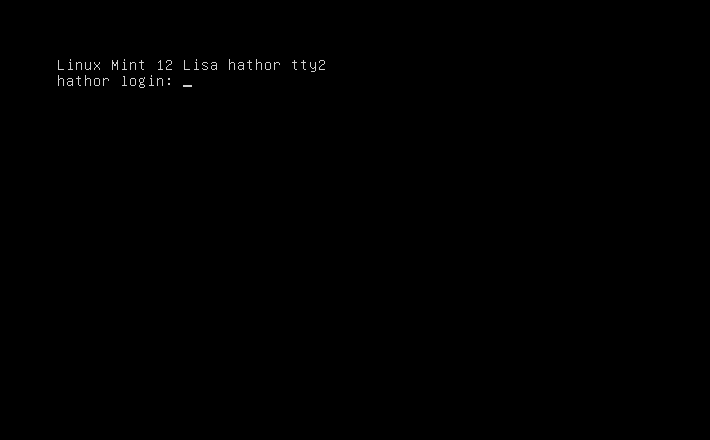
\includegraphics[width=0.7\linewidth,hight=0.7\linehight]{img/tty}
  \end{figure}
\end{frame}

\begin{frame}{Structura unei comenzi}
  \begin{itemize}
    \item comenzi făra argumente
    \begin{itemize}
      \item \cmd{user@host\$ vim}
    \end{itemize}
    \item comenzi cu argumente
    \begin{itemize}
      \item argumentele se separă de comandă prin spațiu
      \item argumentele între ele se separă prin spațiu
      \item unele argumente pot fi flag-uri (precedate de - sau --)
      \item \cmd{user@host\$ ls -a}
      \item \cmd{user@host\$ ls --all}
      \item \cmd{user@host\$ ssh user@remotehost}
      \item \cmd{user@host\$ cp source.file destionation.file}
    \end{itemize}
  \end{itemize}
\end{frame}

\begin{frame}{Exemple de comenzi}
  \input{code/cli-example}
\end{frame}

\begin{frame}{Autocompletion}
  \begin{itemize}
    \item folosind tasta TAB
    \item se completează cel mai lung prefix neambiguu
    \item pentru afișarea sugestiilor se folosește TAB-TAB
  \end{itemize}
\end{frame}

\section{Gestiunea pachetelor}

\begin{frame}{Distribuirea software-ului}
  \begin{itemize}
    \item tarballs (.tar, .tar.gz, .tgz)
    \begin{itemize}
      \item conțin surse, trebuiesc compilate
      \item necesită un toolchain pentru compilare
      \item sunt independente de platformă
      \item ``the Slackware way''
    \end{itemize}
    \pause
    \item package manager (.rpm, .deb)
    \begin{itemize}
      \item construite pentru o arhitectură/distribuție
      \item simplitate în administrare
      \begin{itemize}
        \item controlul versiunilor
        \item controlul dependențelor și al conflictelor
      \end{itemize}
    \end{itemize}
  \end{itemize}
\end{frame}

\begin{frame}{Debian Package Manager}
  \begin{itemize}
    \item folosit pe distribuții bazate pe Debian (inclusiv Ubuntu)
    \item pachet distribuit sub formă de fișier \texttt{.deb}
    \item \texttt{sendmail\_8.12.3-6.6.deb}
    \begin{itemize}
      \item sendmail -- numele pachetului
      \item 8.12.3 -- versiunea pachetului
      \item 6.6 -- versiunea distribuției pentru care este pachetul
    \end{itemize}
    \item utilitare
    \begin{itemize}
      \item dpkg
      \item apt-get
      \item apt-cache
      \item Synaptic, Aptitude
    \end{itemize}
  \end{itemize}
\end{frame}

\begin{frame}{APT (Advanced Packaging Tool)}
  \begin{itemize}
    \item caută și instalează pachete din locații specificate
    (\textbf{repositories})
    \item \texttt{/etc/apt/sources.list}
    \item \texttt{apt-get}
    \begin{itemize}
      \item update -- actualizează lista de pachete disponibile
      \item install -- instalează un pachet
      \item remove -- șterge un pachet
      \item uprade -- instalează o versiune mai nouă a unui pachet
    \end{itemize}
    \item mai nou \texttt{aptitude}
    \item \texttt{apt-cache}
    \begin{itemize}
      \item search -- caută un șir de caractere în numele și descrierile
      pachetelor din baza de date
    \end{itemize}
  \end{itemize}
\end{frame}

\begin{frame}{dpkg}
  \begin{itemize}
    \item back-end-ul folosit de \texttt{apt}
    \item folosit pentriu instalarea unor fișiere \texttt{.deb} (din afara
      repository-urilor)
    \item folosit pentru interogarea bazei de date locale cu pachete
      \begin{itemize}
        \item \texttt{dpkg -l '*alf*'} -- listează pachetele ce conțin șirul
          alf
        \item \texttt{dpkg -L procps} -- afișează fișierele din sistem care au
          fost instalate din cadrul pachetului \texttt{procps}
        \item \texttt{dpkg -S /usr/bin/which} -- din ce pachet face parte
          fișierul \texttt{/usr/bin/which}
      \end{itemize}
  \end{itemize}
\end{frame}


\section{Concluzie}

\begin{frame}{Cuvinte cheie}
  \begin{columns}
    \begin{column}[l]{0.5\textwidth}
      \begin{itemize}
        \item sistem de operare
        \item kernel
        \item Linux
        \item distribuții
      \end{itemize}
    \end{column}
    \begin{column}[l]{0.5\textwidth}
      \begin{itemize}
        \item autocompletion
        \item \texttt{apt-get}
        \item \texttt{/etc/apt/sources.list}
        \item \texttt{dpkg}
      \end{itemize}
    \end{column}
  \end{columns}
\end{frame}

\begin{frame}{Resurse utile}
  \begin{itemize}
    \item \url{http://distrowatch.com/}
    \item \url{http://www.kernel.org/}
    \item \url{http://www.debian.org/}
  \end{itemize}
\end{frame}


\section{Întrebări}

\end{document}
